\subsection{A Learned World Model on a Serial Supply Chain}
\label{section:fc_supply_chain}

The cobweb and fishery simulations in Section~\ref{section:fc_dual_sim} use low-dimensional states and structured model classes. The supply-chain simulation instead uses a neural world model on the full physical state. The environment is a two-echelon serial inventory system in which an upstream supplier replenishes a retailer. Its independent demand, linear costs, and full backlogging match key assumptions under which \citet{ClarkScarf1960inventory} derive an echelon base-stock policy form. Deep reinforcement learning has also been deployed for large-scale inventory decisions \citep{Madeka2022DeepInventory}. Across lost-sales, dual-sourcing, and multi-echelon problems, \citet{Gijsbrechts2022inventory} find that A3C can match specialized heuristics but does not uniformly outperform them.

The retailer at stage one faces Poisson demand with mean five and backorders any unmet demand. Both stages place orders each period, and every shipment has a one-period lead time. The upstream stage fills the retailer's order from available inventory and backlogs any shortfall. The period cost is installation holding at both stages plus a customer-backorder penalty at the retailer. The six-dimensional observation contains on-hand inventory and one in-transit shipment at each stage, the internal backlog, and the customer backorder. The Clark-Scarf policy uses the two echelon inventory positions, while the DQN receives only the six raw state variables. Each of the five methods is evaluated for five hundred steps on the same twenty seeds. No learner is told the true demand rate or the cost coefficients. The neural world-model planner and naive rule estimate customer demand from observations, while the decentralized heuristic estimates each stage's local inflow. The DQN instead learns action values directly from observed transitions without an explicit demand-rate estimate. The benchmark applies the echelon base-stock policy of \citet{ClarkScarf1960inventory}, with levels selected by coordinate search on simulated demand from the true environment. Regret is measured relative to this policy. In the one-stage specialization, the selected level lies within one unit of the closed-form newsvendor base-stock. The neural world model predicts the change in observed state and the normalized reward from the current state, the order vector, and realized demand. At regular intervals, it compares echelon base-stock levels by rolling the network forward under demand resampled from its observations. Unlike MBPO, which generates short policy-training rollouts from replay states \citep{janner2019model}, this planner uses model rollouts to compare policies within a supplied base-stock class. The planner receives the base-stock policy class and the echelon transformation. Once it has observed demand, it initializes the search from estimated mean demand over one protection interval for each echelon depth. The model-free deep Q-network estimates action values from the raw physical state over a grid of twenty-five joint order actions. The decentralized heuristic runs a local base-stock at each stage from its own observed inflow, ignoring the echelon coupling, and the naive rule orders its running mean of observed demand every period.

Table~\ref{table:fc_supply_chain} reports cumulative regret against the benchmark and the terminal per-period cost over the last eighty steps, and Figure~\ref{figure:fc_supply_chain} shows the regret trajectories and the world model's one-step forecast error over training. Cumulative regret includes the full five hundred steps. Terminal cost is the mean per-period cost over the final eighty steps. The world model's terminal cost is 8.00, compared with 6.61 for the benchmark and 9.84 for the decentralized heuristic. Its terminal cost is therefore 21 percent above the benchmark. The decentralized heuristic has lower cumulative regret than the world model, 1965 against 3879. The world model samples exploratory base-stock targets during its first fifty steps and later adds decaying action noise, while the decentralized heuristic does not add exploration noise. The naive rule records cumulative regret of 29,485 and terminal cost of 106.05. The configured DQN records cumulative regret of 44,137 and terminal cost of 210.79. Both have higher cumulative regret and terminal cost than the decentralized and world-model policies within the five hundred step budget. For seed zero, the plotted rolling mean of one-step state forecast MSE begins above ten and ends near 0.3. This comparison does not isolate model-based from model-free learning. The world model receives the base-stock policy class and the echelon transformation, whereas the DQN estimates values from the raw physical state. The terminal-cost ranking is consistent with \citet{Gijsbrechts2022inventory}, who find that A3C can match specialized inventory heuristics without uniformly outperforming them. Since the benchmark's base-stock levels come from simulation-based coordinate search, these results do not establish a globally optimal cost.

\begin{figure}[ht]
  \centering
  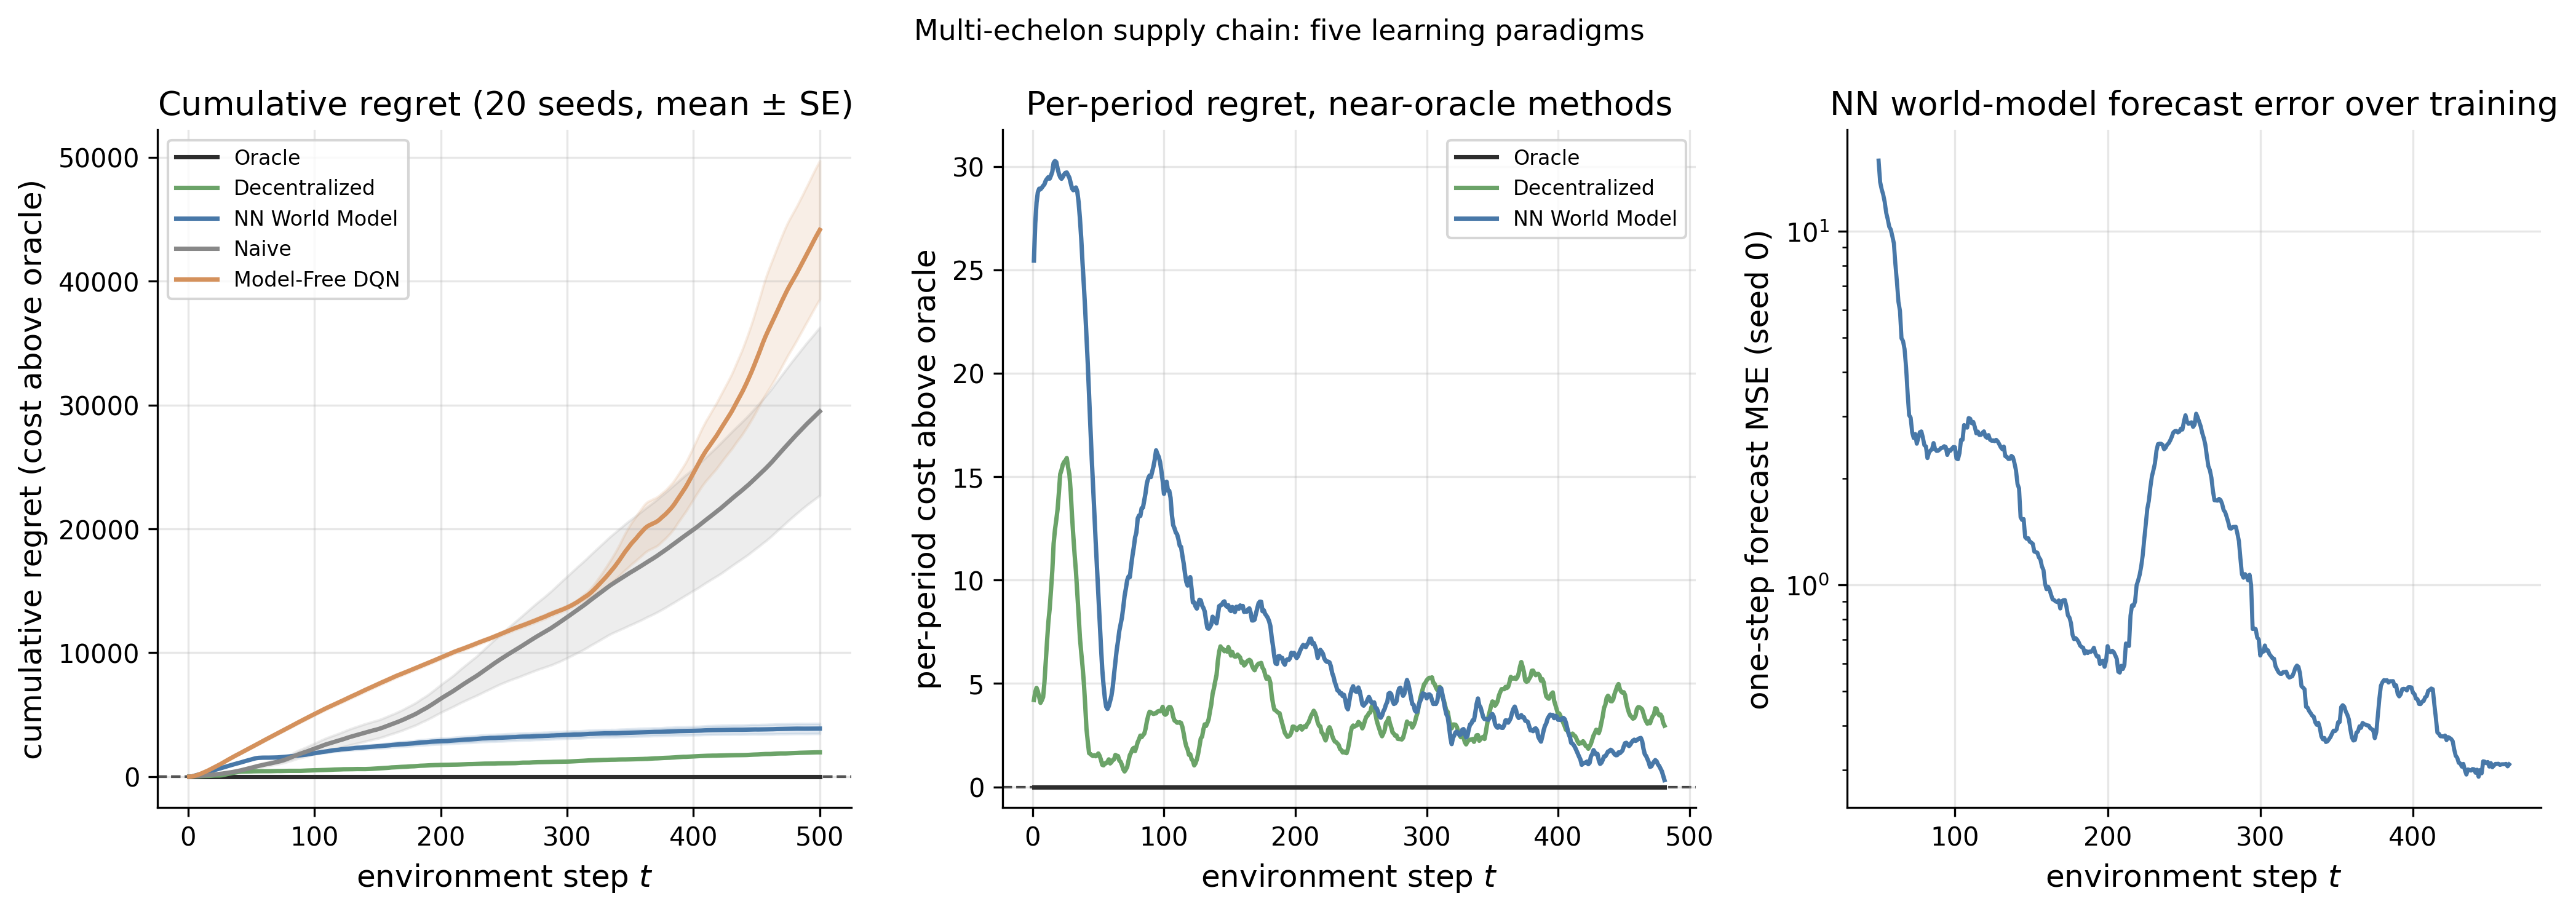
\includegraphics[width=\textwidth]{../ch12_world_models/sims/multi_echelon_paradigms.png}
  \caption{Cumulative regret relative to the Clark-Scarf benchmark appears in the left panel, with means and one-standard-error bands over twenty seeds. The middle panel gives the twenty-step moving average of per-period regret for the benchmark, decentralized heuristic, and neural world model. The right panel gives a rolling mean of the neural world model's one-step state forecast MSE for seed zero on a logarithmic scale.}
  \label{figure:fc_supply_chain}
\end{figure}

\begin{table}[ht]
  \centering
  \caption{Cumulative regret relative to the Clark-Scarf benchmark at $T=500$ and terminal per-period cost over the final eighty steps, mean $\pm$ standard error across twenty seeds. Methods are ordered by cumulative regret, and lower values indicate lower cost. The benchmark is the zero-regret reference and has terminal cost 6.61.}
  \label{table:fc_supply_chain}
  % Cumulative regret vs Clark-Scarf oracle at T=500 and terminal per-period cost (last 80 steps), mean +- SE over 20 seeds.
\begin{tabular}{lrr}
\toprule
Paradigm & Cumulative regret & Terminal cost/period \\
\midrule
Oracle & 0.0 $\pm$ 0.0 & 6.61 $\pm$ 0.17 \\
Decentralized & 1964.8 $\pm$ 50.8 & 9.84 $\pm$ 0.26 \\
NN World Model & 3879.4 $\pm$ 406.5 & 8.00 $\pm$ 0.88 \\
Naive & 29485.4 $\pm$ 6777.2 & 106.05 $\pm$ 29.04 \\
Model-Free DQN & 44137.1 $\pm$ 5593.1 & 210.79 $\pm$ 53.76 \\
\bottomrule
\end{tabular}

\end{table}
